% chktex-file 1
\documentclass{article}
% chktex-file 34
% chktex-file 18
% chktex-file 1
\usepackage{amsfonts}
\usepackage[T1]{fontenc}
\usepackage{amsmath}
\usepackage{amssymb}
\usepackage{mathrsfs}
\usepackage{extarrows}
\usepackage{hyperref}
\usepackage[utf8]{inputenc}
\usepackage{graphicx}
\usepackage{mathtools}
\usepackage[a4paper, total={6in, 8in}]{geometry}
\usepackage[table]{xcolor}
\usepackage{tikz}
\usepackage{cancel}
\usepackage{steinmetz}
\usepackage{diagbox}
\usepackage{siunitx}
\usepackage{eurosym}
\usepackage{pgfplots}
\pgfplotsset{width=10cm,compat=1.9}
\usetikzlibrary{shapes,arrows}
\usepackage{listings}
\usepackage{color}
%definizione colori per blocchi di codice
\definecolor{lightgray}{rgb}{.95,.95,.95}
\definecolor{darkgray}{rgb}{.4,.4,.4}
\definecolor{purple}{rgb}{0.65, 0.12, 0.82}
\definecolor{ocherCode}{rgb}{1, 0.5, 0}
\definecolor{blueCode}{rgb}{0, 0, 0.93}
\definecolor{greenCode}{rgb}{0, 0.6, 0}

%formattazione per i blocchi di codice
\lstset{
  %Special characters
  literate={á}{{\'a}}1 {é}{{\'e}}1 {í}{{\'\i}}1 {ó}{{\'o}}1 {ú}{{\'u}}1 {Á}{{\'A}}1 {É}{{\'E}}1 {Í}{{\'I}}1 {Ó}{{\'O}}1 {Ú}{{\'U}}1 {à}{{\`a}}1 {è}{{\`e}}1 {ì}{{\`\i}}1 {ò}{{\`o}}1 {ù}{{\`u}}1 {À}{{\`A}}1 {È}{{\`E}}1 {Ì}{{\`I}}1 {Ò}{{\`O}}1 {Ù}{{\`U}}1 {ä}{{\"a}}1 {ë}{{\"e}}1 {ï}{{\"\i}}1 {ö}{{\"o}}1 {ü}{{\"u}}1 {Ä}{{\"A}}1 {Ë}{{\"E}}1 {Ï}{{\"I}}1 {Ö}{{\"O}}1 {Ü}{{\"U}}1 {â}{{\^a}}1 {ê}{{\^e}}1 {î}{{\^\i}}1 {ô}{{\^o}}1 {û}{{\^u}}1 {Â}{{\^A}}1 {Ê}{{\^E}}1 {Î}{{\^I}}1 {Ô}{{\^O}}1 {Û}{{\^U}}1 {ã}{{\~a}}1 {ẽ}{{\~e}}1 {ĩ}{{\~\i}}1 {õ}{{\~o}}1 {ũ}{{\~u}}1 {Ã}{{\~A}}1 {Ẽ}{{\~E}}1 {Ĩ}{{\~I}}1 {Õ}{{\~O}}1 {Ũ}{{\~U}}1 {œ}{{\oe}}1 {Œ}{{\OE}}1 {æ}{{\ae}}1 {Æ}{{\AE}}1 {ß}{{\ss}}1 {ű}{{\H{u}}}1 {Ű}{{\H{U}}}1 {ő}{{\H{o}}}1 {Ő}{{\H{O}}}1 {ç}{{\c c}}1 {Ç}{{\c C}}1 {ø}{{\o}}1 {Ø}{{\O}}1 {å}{{\r a}}1 {Å}{{\r A}}1 {€}{{\euro}}1 {£}{{\pounds}}1 {«}{{\guillemotleft}}1 {»}{{\guillemotright}}1 {ñ}{{\~n}}1 {Ñ}{{\~N}}1 {¿}{{?`}}1 {¡}{{!`}}1 {'"'}{\textquotesingle "\textquotesingle}3,
  %Basic design
  backgroundcolor=\color{lightgray},
  frame=l,
  % Line numbers
  xleftmargin={0.75cm},
  numbers=left,
  numberstyle=\footnotesize,
  numbersep=9pt,
  stepnumber=1,
  firstnumber=1,
  numberfirstline=true,
  % Code design
  identifierstyle=\color{black},
  keywordstyle=\color{blue}\bfseries,
  ndkeywordstyle=\color{ocherCode}\bfseries,
  stringstyle=\color{greenCode}\ttfamily,
  commentstyle=\color{darkgray}\ttfamily,
  %Code
  columns=[c]fixed,
  extendedchars=true,
  upquote=true,
  breaklines=true,
  showstringspaces=false,
  showspaces=false,
  tabsize=2,
  breaklines=true,
  showtabs=false,
  captionpos=b
}
%lingue supportate:
%ABAP
%ACSL
%Ada
%Algol
%Ant
%Assembler
%Awk
%bash
%Basic
%C#5
%C++
%C
%Caml
%Clean
%Cobol
%Comal
%csh
%Delphi
%Eiffel
%Elan
%erlang
%Euphoria
%Fortran
%GCL
%Go (golang)
%Gnuplot
%Haskell
%HTML
%IDL
%inform
%Java
%JVMIS
%ksh
%Lisp
%Logo
%Lua
%make
%Mathematica
%Matlab
%Mercury
%MetaPost
%Miranda
%Mizar
%ML
%Modelica
%Modula-2
%MuPAD
%NASTRAN
%Oberon-2
%Objective C
%OCL
%Octave
%Oz
%Pascal
%Perl
%PHP
%PL/I
%Plasm
%POV
%Prolog
%Promela
%Python
%R
%Reduce
%Rexx
%RSL
%Ruby
%S4
%SAS
%Scilab
%sh
%SHELXL
%Simula
%SQL
%tcl4
%TeX
%VBScript
%Verilog
%VHDL
%VRML
%XML
%XSLT

\newcommand{\acapo}{\\\hspace*{1cm}\\}
\newcommand{\Eaccentata}{$\grave{\text{E}}$ }
\newcommand{\vopen}{``}
\newcommand{\apexopen}{`}
\newcommand{\vclose}{''}
\newcommand{\vclosespace}{'' }
\newcommand{\indenta}{\hspace*{1cm}}
\newcommand{\define}{\underline{Def:} }

\setlength{\parindent}{0cm}

\hfuzz=100pt

\author{Flavio Colacicchi}

\title{Processi software\\\normalsize Analisi e progettazione del software}
\date{06\textendash11/03/2025}
\begin{document}
\maketitle
Un processo software definisce dei ruoli, ovveri chi fa cosa, quando e come per raggiungere un certo obiettivo e opera seguendo una timeline di attività comuni nei processi software:
\begin{enumerate}
    \item Specifica (o analisi) dei requisiti
    \item Analisi
    \item Progettazione
    \item Implementazione
    \item Validazione e verifica
    \item Rilascio/Installazione
    \item Manutenzione/evoluzione
    \item Gestione del progetto
\end{enumerate}
Esistono divenrsi processi software e si differenziano soprattutto per l'organizzazione temporale delle attività, in particolare nell'ordine delle attività e nei criteri di transizioni da un'attività a un'altra.\acapo
\textbf{Processo a cascata}, un processo classico ancora molto diffuso e definito negli anni \apexopen60/\apexopen70, in questo processo le attività sono svolte in maniera sequenziale:
\begin{enumerate}
    \item Pianificazione
    \item Analisi dei requisiti del softwareProgettazione
    \item Implementazione del codice
    \item Collaudo
\end{enumerate}
Spesso queste attività sono svolte da team differenti che producono documenti dettagliati con le attività le quali possono procedere solo dopo aver convalidato i documenti dell'attività precedente. Questa tipologia di rpocesso ha origine a partire dall'ingegneria civile e nalla maggior parte dei casi non funziona bene per lo sviluppo software per una serie di motivi:
\begin{itemize}
  \item Un'ipotesi fondamentale è poter definire correttamente e congelare i requisiti prima di poter procedere con le fasi successive, il che è un'ipotesi irrealistica
  \item Tutte le \vopen buone idee\vclosespace dovrebbero venire fuori prima dello sviluppo senza poter poi implementare idee nuove
  \item Non consente una gestione efficace dei rischi
\end{itemize}
Per ovviare a questi problemi sono nate altre tipologie di processi di sviluppo, ad esempio lo \textbf{sviluppo ecolutivo} dove si fa una realizzazione iniziale del sistema e la si espone agli utenti pe rottenere un feedback al fuine di raffinare l'implementazione, una forma di svilippo evolutivo è lo \textbf{sviluppo iterativo} dove si lavora in iterazioni di breve dirata fissa (ad esempio 2\textendash4 settimane) all'interno delle quali si svolgono attività di analisi, progettazione, implementazione anche se parziale e test per ottenere feedback e ripetere le iterazioni per migliorare la qualità del prodotto aumentando lla quantità di funzioni nel tempo e completare il software e questo porta una serie di vantaggi:
\begin{itemize}
  \item minor probabilità di fallimento del progetto
  \item Miglior probabilità
  \item Minor probabilità di difetti
  \item Riduzione precoce anziché tardiva dei rischi
  \item Visibilità del progresso
  \item Feedback precoce
  \item Impegno degli utenti
  \item Adattamento
  \item Gestione della complessità
  \item Miglioramento continuo del processo stesso
\end{itemize}
E rischi:
\begin{itemize}
  \item Gestione del tempo
  \item In che ordine considero i requisiti
  \item Gestione pratica dei cambiamenti
\end{itemize}
Per affrontare i rischi ci sono diverse strategie, ad esempio il timeboxing dove ogni iterazione deve avere una durata prefissata così da avere un feedback continuo.\\
Nello sviluppo iterativo è importante che il software possegga alcune quelità:
\begin{itemize}
  \item Flessibile
  \item Modificabile
  \item Comprensibile
\end{itemize}
\textbf{Unified Process} (UP) è un processo \textbf{iterativo} per lo sviluppo di software OO che promuove diverse best practice:
\begin{itemize}
  \item Sviluppare software in modo iterativo, evolutivo ed adattivo
  \item Sviluppo guidato dal rischio
  \item Sviluppare il cuore dell'architettura nelle prime iterazioni
  \item \dots
\end{itemize}
Nel quale ogni iterazione è divisa in 4 fasi composte da diverse iterazioni:
\begin{center}
  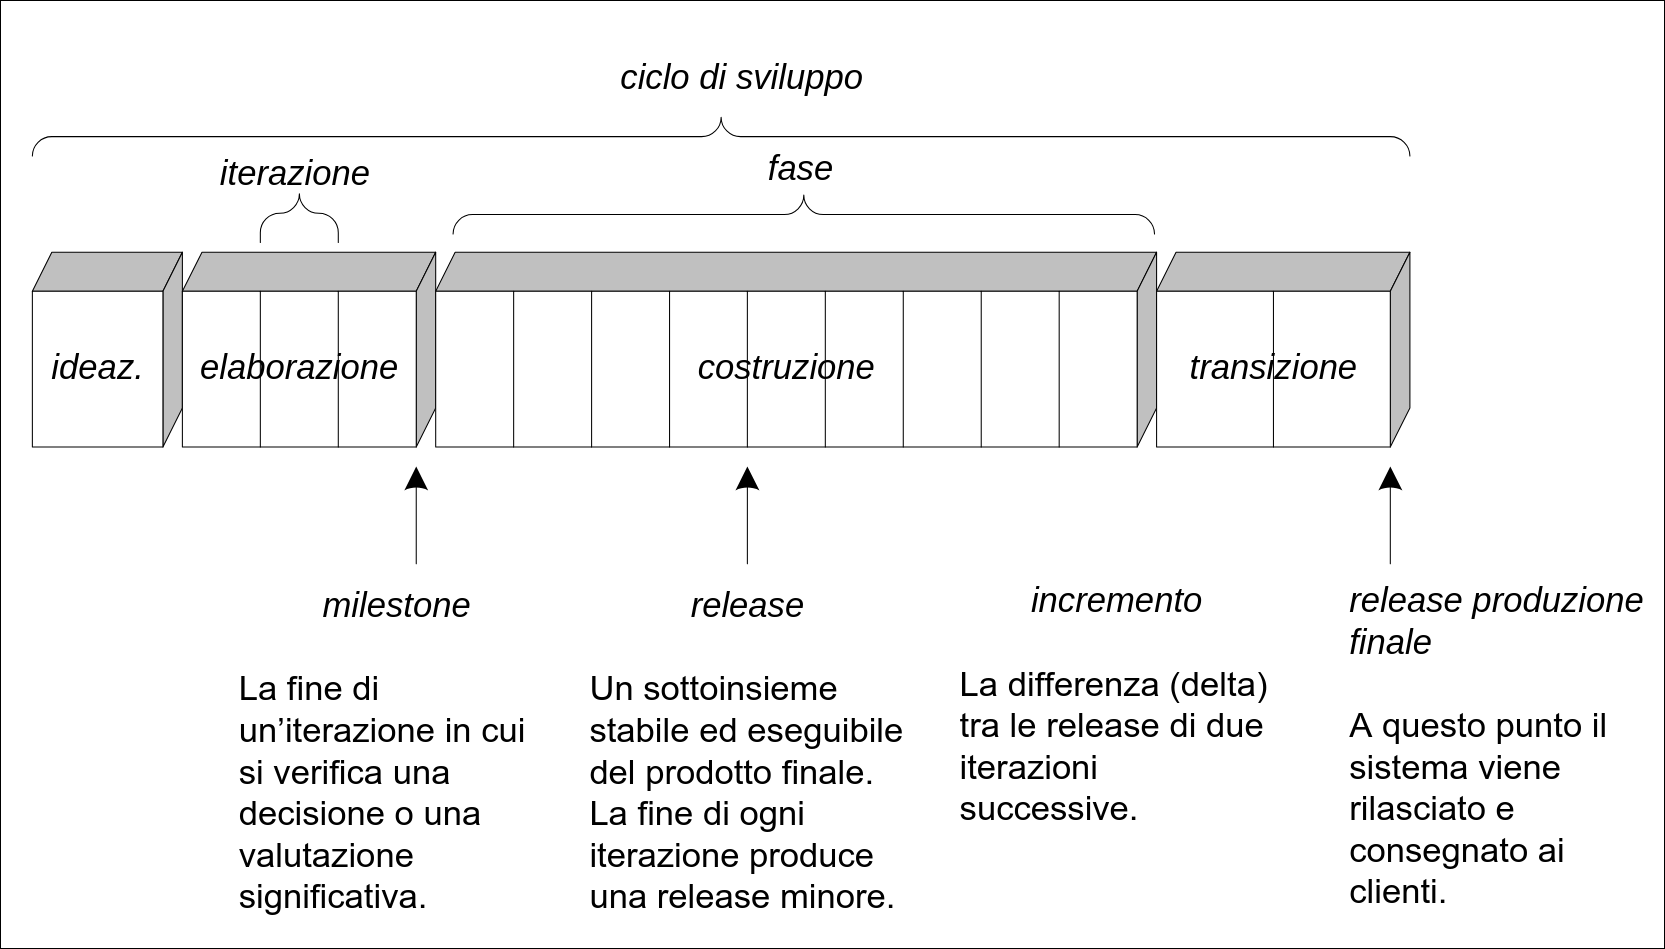
\includegraphics[width=10cm]{images/fasi up.png}
\end{center}
\begin{enumerate}
  \item Ideazione:\\
        in genere molto preve dove si identificano i primi requisiti
  \item Elaborazione:\\
        iterazioni in cui si crea il nucleo del progetto
  \item Costruzione:\\
        Dove viene svolta la maggior parte del alvoro e vengono implementati la maggioranza dei requisiti
  \item Transizione
\end{enumerate}
Le varie discipline di UP hanno un peso diverso lungo il processo
\begin{center}
  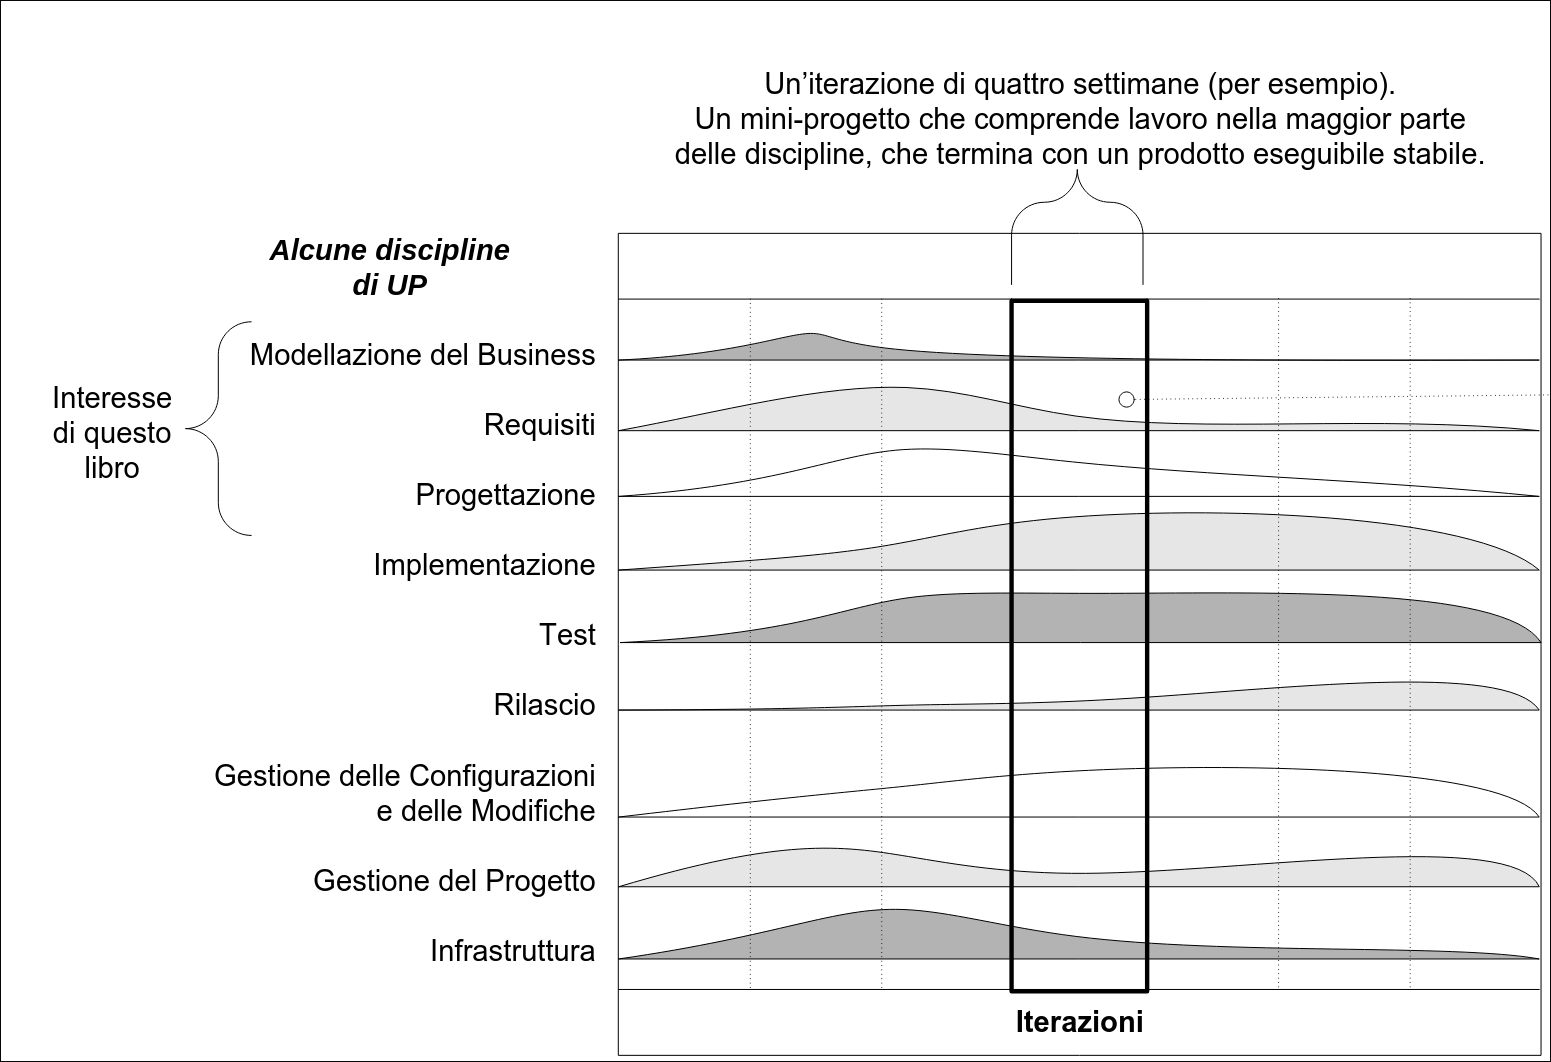
\includegraphics[width=10cm]{images/discipline up nello sviluppo.png}
\end{center}
\newpage
Un metodo \textbf{agile} è una forma di sviluppo iteragtivo in grado di rispondere in modo rapido e flessibile ai cambiamenti.\acapo
Nello sviluppo vi è una breve iterazione 0 in cui abbiamo una prima analisi dei beneifici ma l'attività più importante di questa iterazione è l'analisi economica del bilancio costi\textendash benefici
\end{document}